\begin{atiTask}[
  title = Vektoroperatoridentitäten II
  %call = Zusatzaufgabe,
]
%SoSe17 blatt 5 /5 
Bestätigen Sie im Indexkalkül die Identitäten
\begin{atiSubequations}
\item{\vec{c}\gradient (\vec{a}\vec{b})=\vec{a}(\vec{c}\gradient)\vec{b}+\vec{b}(\vec{c}\gradient)\vec{a}}
%
\item{(\vec{c}\gradient)(\vec{a}\times \vec{b})=\vec{a}\times (\vec{c}\gradient )\vec{b}-\vec{b}\times (\vec{c}\gradient)\vec{a}}
%
\item{(\nabla \vec{a})\vec{b}=(\vec{a}\gradient)\vec{b}+\vec{b}\divergence \vec{a}}
%
\item{(\vec{a}\times \vec{b})\curl \vec{c}=\vec{b}(\vec{a}\gradient)\vec{c}-\vec{a}(\vec{b}\gradient)\vec{c}}
%
\item{(\vec{a}\times \gradient)\times \vec{b}=(\vec{a}\gradient)\vec{b}+\vec{a}\times \curl \vec{b}-\vec{a}\divergence \vec{b}}
%
\item{(\nabla\times\vec{a})\times\vec{b}=\vec{a}\divergence \vec{b}-(\vec{a}\gradient)\vec{b}-\vec{a}\times \curl \vec{b}-\vec{b}\times \curl \vec{a}}
%
\end{atiSubequations}
\atiNote{Beachten Sie, dass der Nabla-Operator $\mathbf{\nabla}$ in den Beispielen (iii) und (vi) auf \textit{beide} rechts von ihm stehende Vektorfelder wirken soll.}


\end{atiTask}

\begin{atiSolution}
	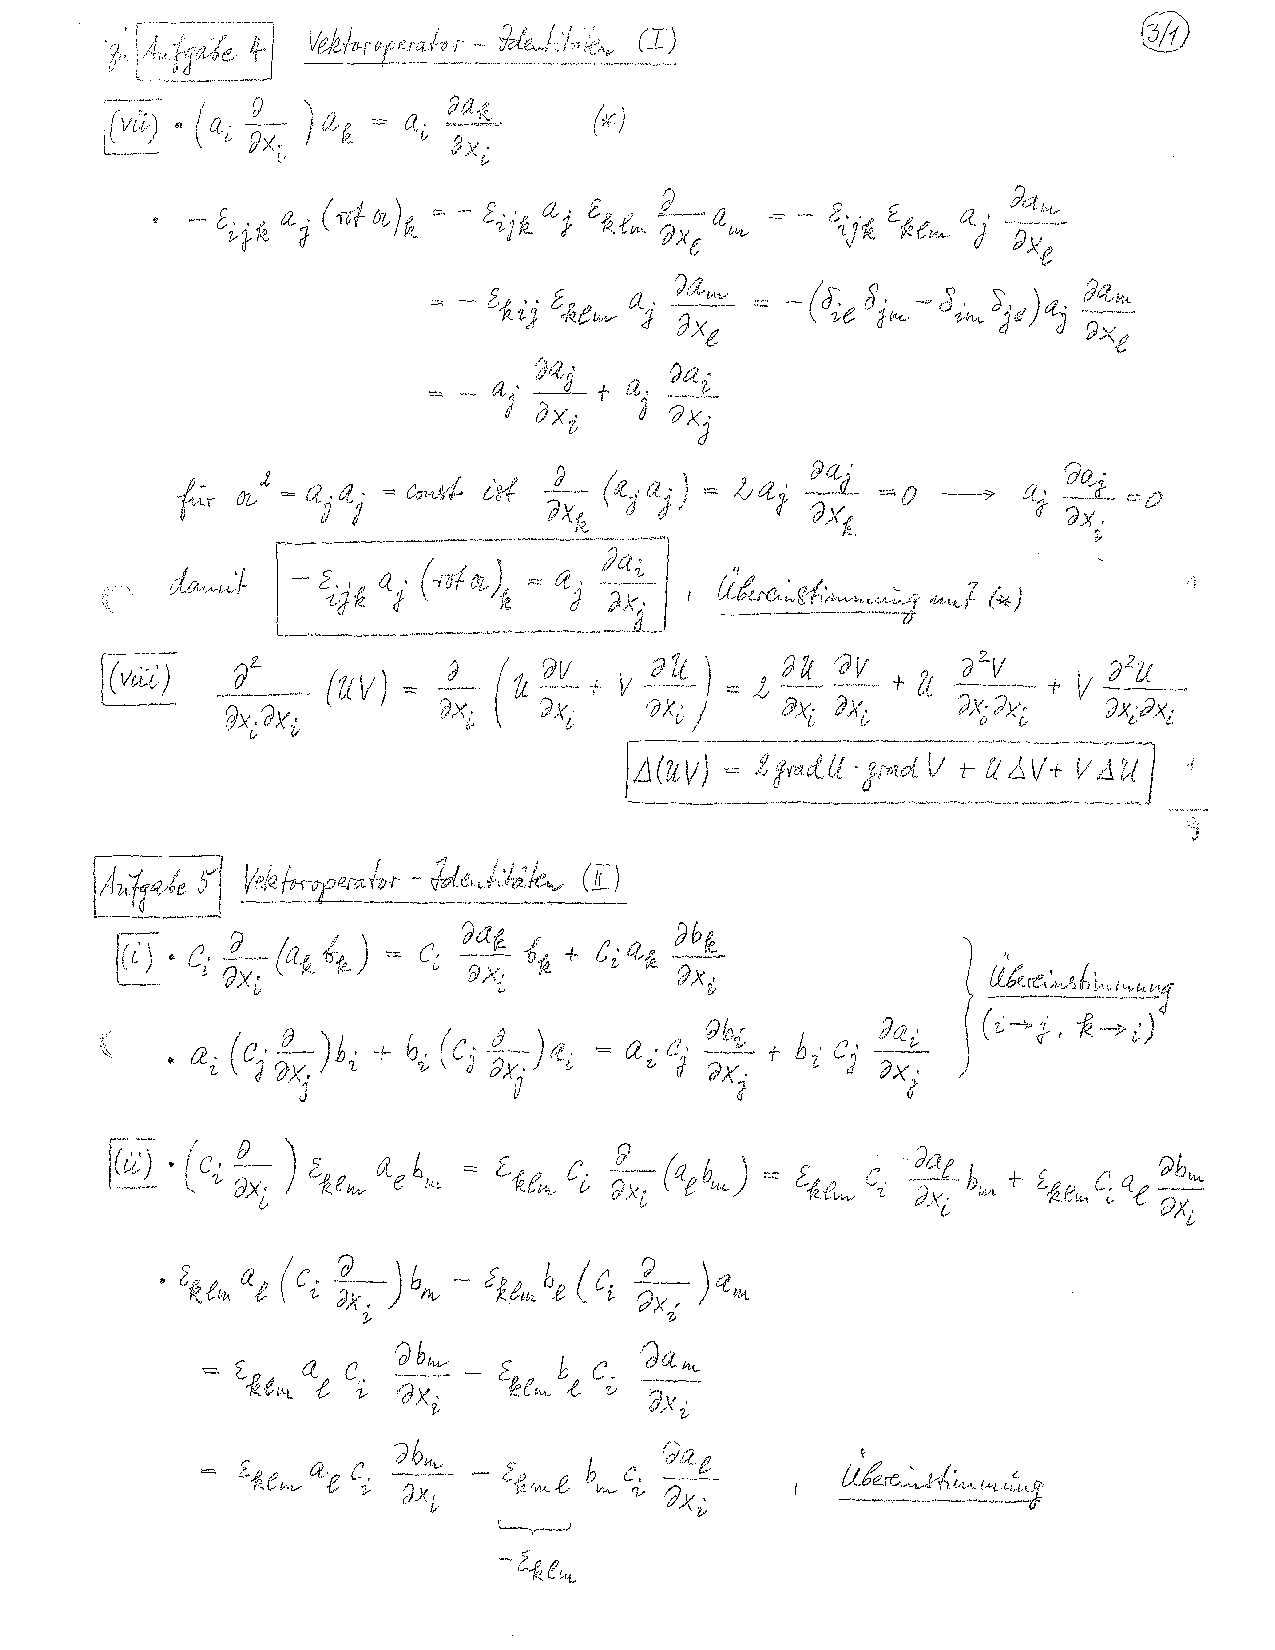
\includepdf{solution-index_ii.pdf}
\end{atiSolution}